

\section{Componentes Eletrônicos 3}
\label{componentes_3}


\begin{table}[ht!]

	\begin{tabular}{r l|l p{12cm} }
		
		\textcolor{gray}{Especificação} &&& 	{Componentes Eletrônicos 3}\\
		\textcolor{gray}{Data} &&& 				{28/05/2014}\\
        \textcolor{gray}{Beneficiado} &&&		{TMP 2003 COM. Eletro Eletron. LTDA}
        \\
        \textcolor{gray}{CNPJ} &&& 				{07.976.241/0001-10} \\
        \textcolor{gray}{Número Nota} &&& 		{6543} \\
		\textcolor{gray}{Quantidade} &&& 		{-} \\
		\textcolor{gray}{Valor} &&& 			{R\$84,00} \\
		\textcolor{gray}{Data Sheet} &&& 		{-} \\

		\textcolor{gray}{Função no projeto} &&& {Os componentes eletrônicos 3 são
		compostos por : reguladores, capacitores, barra sindal, barra de pino,
		adaptador de tomada, extensão de 5 metros. Com exceção dos adaptadores de
		tomada e a extensão, que foram adquiridos para a viagem em Jirau (Maio), os
		componentes são necessários para testes da eletrônica. Os reguladores são
		necessários para converter voltagem de alimentação até o nível de operação
		3.3V e 5V, capacitores são usados para filtros de alguns
		dispositivos analógicos, barra sindal possibilitam teste rápido de conexões
		sem a necessidade de solda e as barras de pino são utilizadas na protoboard ou
		placa customizada para plugs de baixa corrente.}
		\\
		\textcolor{gray}{Razão da Escolha} &&& {-}

	\end{tabular}
\end{table}

\newpage


\subsection{Nota Fiscal}
\begin{figure}[H]
 \centering
 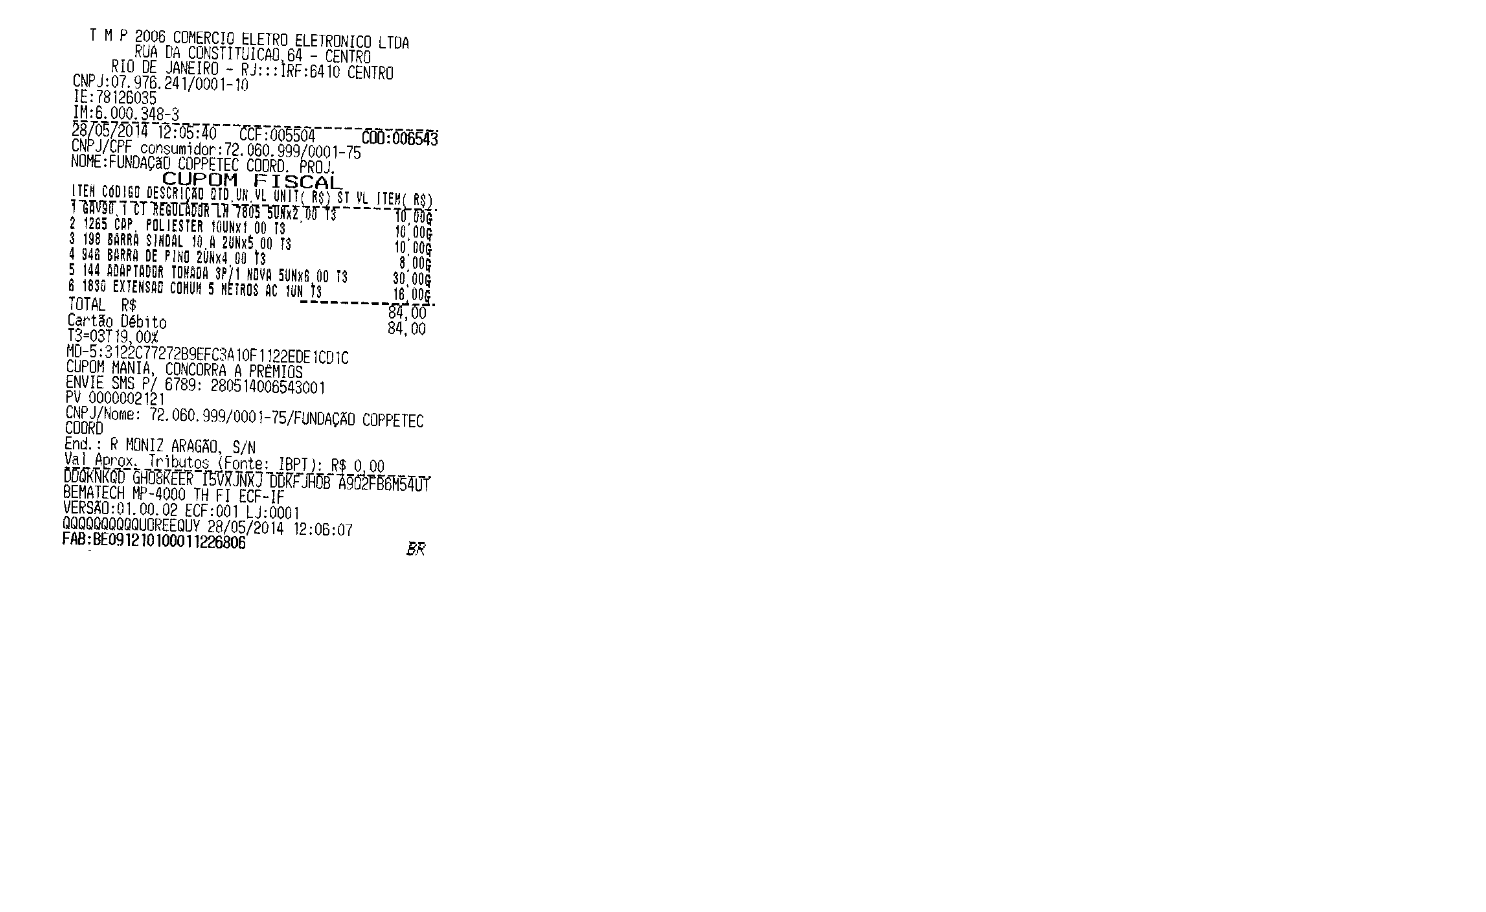
\includegraphics[width=1\columnwidth]{Componentes_Eletronicos_3/nota_eletronica3.png}
 \caption{Componentes Eletrônicos 3}
 \end{figure}